\newpage \section{van der Meer calibration}
\label{sec:vdm}
Van der Meer (VdM) scans are done to calculate the visible cross section $\sigma_{vis}$ which is a calibration constant in the relation between rate of a quantity (clusters, coincidences) read out by the detector and the instantaneous luminosity. \\

The instantaneous luminosity when the crossing angle between the colliding bunches is negligible and bunches collide head on is given by the following integral, \\

L = N_1 N_2 f \int^{+\infty}_{-\infty} \rho_1(x,y) \rho_2(x+\Delta x, y+ \Delta y) dx dy \\

where $N_1, N_2$ are the number of protons in the colliding bunches, f is the LHC orbit frequency whose value is 11246Hz,  $\rho_1(x,y)$ and $\rho_2(x+\Delta x,y+\Delta y)$ are the two dimensional particle density distribution functions for each colliding bunch separated by $\Delta x$ and $\Delta y$ in the x and y directions. \\

Assuming complete factorization of particle density distribution function along x and y directions for both the bunches, we get \\

L = N_1 N_2 f \int^{+\infty}_{-\infty} \rho_{1x}(x) \rho_{2x}(x+\Delta x)  dx   \int^{+\infty}_{-\infty} \rho_{1y}(y) \rho_{2y}(y+\Delta y)  dy \\

where $\rho_1(x,y) = \rho_{1x}(x,y) \rho_{1y} (x,y)$ and $\rho_2(x+\Delta x,y + \Delta y) = \rho_{2x}(x+\Delta x,y+\Delta y) \rho_{2y} (x+\Delta,y+\Delta y)$ \\

The VdM scan determines the bunch  overlap integrals $\int \rho_{x1} (x) \rho_{x2} (x+\Delta x) dx$ and  $\int \rho_{y1}(y) \rho_{y2} (y+\Delta y) dy$ by measuring pixel clusters rate as a function of bunch separation $\Delta x$ and $\Delta y$ along x and y directions as shown in Fig. 7. \\

\int \rho_{x1} (x) \rho_{x2} (x+\Delta x) dx = \frac{R_x(0)}{\int R_x(\Delta x)dx} \\

\int \rho_{y1} (y) \rho_{y2} (y + \Delta y) dy = \frac{R_y(0)}{\int R_y(\Delta y)dy} \\

Bunch overlap widths $\Sigma_x$ and $\Sigma_y$ along x and y directions are defined as \\

\Sigma_x = \frac{1}{\sqrt{2 \pi}} \frac{\int R_x(\Delta x)dx}{R_x(0)} \\

\Sigma_y =  \frac{1}{\sqrt{2 \pi}} \frac{\int R_y(\Delta y)dy}{R_y(0)} \\

$\Sigma_x \Sigma_y = \frac{1}{2 \pi} \frac{\int R_x(\Delta x)dx \int R_y(\Delta y) dy}{R_x(0) R_y(0)}$  is the bunch overlapping area as shown in Fig. 8 by the red region.\\

Thus, the expression for instantaneous luminosity is given by \\

L = $\frac{N_1 N_2 f}{2\pi \Sigma_x \Sigma_y}$ \\

and the PCC visible cross section defined in terms of beam parameters and rate is given by \\

\sigma_{vis} = \frac{2 \pi \Sigma_x \Sigma_y R}{N_1 N_2} \\


\begin{figure}[H]
  \centering
  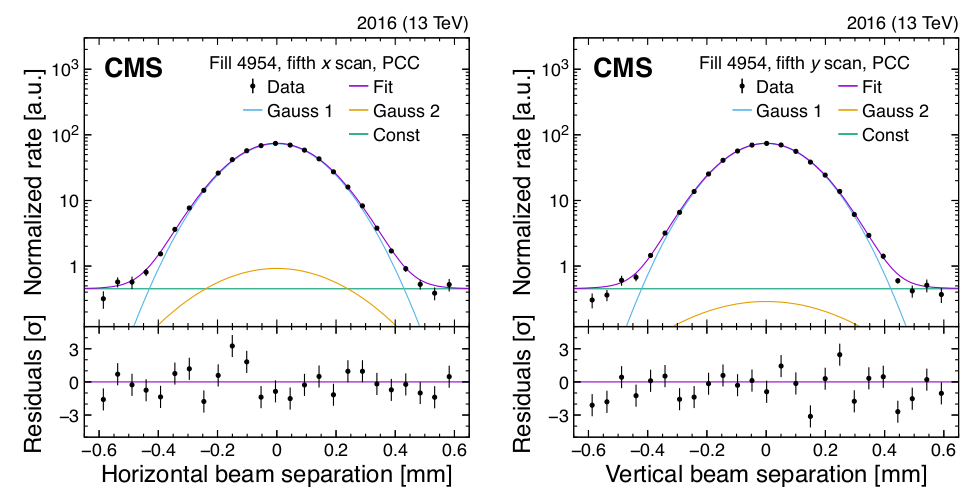
\includegraphics[width=0.7\columnwidth]{./vdmfit.png}
  \caption{ \onehalfspacing Example vdM scans for PCC for BCID 41, from the last scan pair in fill 4954, showing the rate normalized by the product of beam currents as a function of the beam separation $\Delta x$ and $\Delta y$ in the x (left) and y (right) direction, and the fitted curves. The purple curve shows the overall double-Gaussian fit, while the blue, yellow, and green curves show the first and second Gaussian components and the constant component, respectively. The lower panels display the difference between the measured and fitted values
divided by the statistical uncertainty\cite{}.}
  \label{fig:CMS}
\end{figure}


\begin{figure}[H]
  \centering
  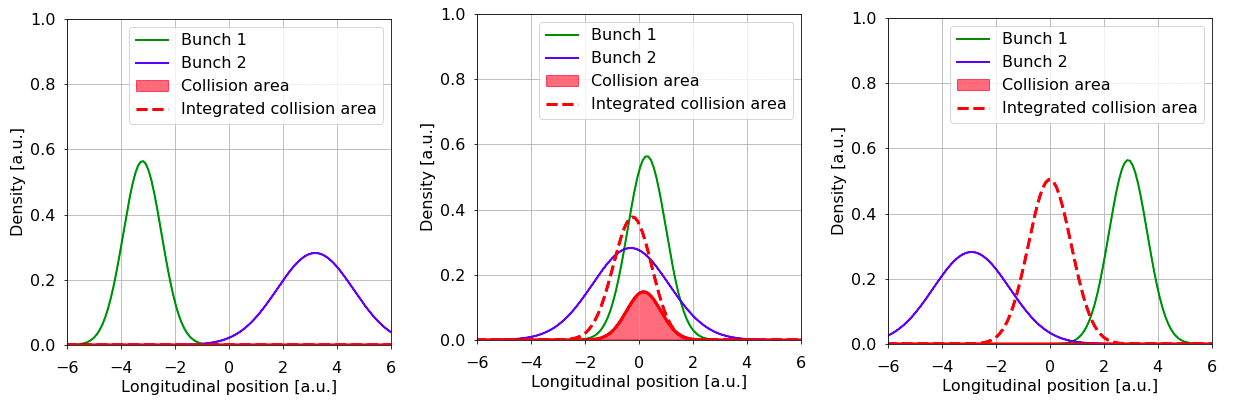
\includegraphics[width=\columnwidth]{./vdm_image.png}
  \caption{\onehalfspacing Figure showing two LHC bunches in green and blue approaching each other and colliding giving rise to an overlapping region showing in red whose area is determined during VdM scans.}
  \label{fig:CMS}
\end{figure}






